\documentclass{beamer}

% Preamble {{{2

\usepackage{etex} % To stop 'No room for a new \dimen' message

\usetheme[base=blue]{cambridge}
\usefonttheme{professionalfonts}

\usepackage{program}
\usepackage[english]{babel}
\usepackage{ifxetex}
\usepackage{listings}
\usepackage{amssymb}
\usepackage{graphicx}

\lstset{
  basicstyle=\ttfamily\footnotesize,
  %identifierstyle=\color{CambridgeCoreBlue},
  commentstyle=\color{CambridgeDarkOrange},
  stringstyle=\color{CambridgeCorePurple},
  directivestyle=\color{CambridgeDarkTeal},
  keywordstyle=\ttfamily\color{CambridgeDarkGreen!25!CambridgeCoreGreen},
  emphstyle=\color{CambridgeDarkTeal!50!CambridgeCoreTeal},
  numbers=left,
  numberstyle=\tiny\color{gray},
  stepnumber=1,
  numbersep=5pt,
  % backgroundcolor=\color{white},
  tabsize=4,
  showspaces=false,
  showstringspaces=false,
}

\lstdefinelanguage{GLSL}[ANSI]{C}{
  morekeywords={vec2,vec3,vec4,uniform,sampler2D},
  emph={texture2D,sqrt,gl\_MultiTexCoord},
}

\lstdefinelanguage{Firtree}[ANSI]{C}{
  morekeywords={vec2,vec3,vec4,kernel,\_\_color,\_\_reduce,sampler,in,out},
  emph={length,dot,sqrt,cos,sin,premultiply,unpremultiply,destCoord,sample,samplerTransform,samplerCoord},
}

\lstdefinelanguage{LLVM}[]{}{
  keywords={int,float,i32,i64,i8.i1,nounwind,readnone,declare,define,ret,call,fmul,fadd,fdiv,inttoptr},
  comment={[l];}
}

\ifxetex
  \usepackage[cm-default]{fontspec}
  \usepackage{xunicode}
  \usepackage{xltxtra}

  \setsansfont{Myriad Pro Light}
  \setmainfont{Times New Roman}
  \setmonofont{Andale Mono}
\else
  \usepackage{times}
  \usepackage[T1]{fontenc}
\fi

\title{The Firtree Framework}

\subtitle{A Dynamic Compilation System for Multi-Core Aware Image Processing}

\author{Dr Rich Wareham}
\institute
{
  Department of Engineering\\
  University of Cambridge
}

\date{Rutherford Appleton Laboratories, November 2009}
\subject{Computer Science}

% Make the current ToC pop up at the beginning of each
% new sub-section
\AtBeginSubsection[] 
{
  \begin{frame}<beamer>{Outline}
    \tableofcontents[currentsection,currentsubsection] 
  \end{frame}
}

% Bundle the part definition, part page and ToC into
% one command
\newcommand{\fancypart}[1]{%
  \part{#1}
  \begin{frame}
    \partpage
  \end{frame}
  \begin{frame}{Outline}
    \tableofcontents
  \end{frame}
}

\newcommand{\fixme}[1]{\color{red}{FIXME: #1}}

% Some convenience macros
\newcommand{\bi}{\begin{itemize}}
\newcommand{\ei}{\end{itemize}}

% }}}2

\begin{document}

\begin{frame}
  \titlepage
\end{frame}

\fancypart{Introduction} % {{{1

\section{About Me}  % {{{2

\begin{frame}{About Me}
  \bi
  
  \item Postdoc in the Signal Processing and Communications
  Laboratory\footnote{\url{http://www-sigproc.eng.cam.ac.uk/}}, Department of
  Engineering, University of Cambridge

  \item Member of the Many Core Computing
  Group\footnote{\url{http://www.many-core.group.cam.ac.uk/}} in Cambridge

  \item Have a weakness for writing DSLs

  \ei
\end{frame}

% }}}2

\section{The Firtree Project} % {{{2

\begin{frame}{The Firtree Project}
  \bi
    \item Developed by one man (me!)
    
    \item Personal project developed after I wrote a Sobel filter for the 30th
    time

    \item Hosted at \url{http://firtree.org/}

    \item Aim is to allow me to write once, use many times

    \item An exercise in an intrinsically multi-core capable system
  \ei
\end{frame}

% }}}2

\section{Requirements} % {{{2

\begin{frame}{Requirements}
  \bi

  \item Implemented image processing algorithms in C

  \item Want to make use of multi-core hardware

  \item Don't want to be fussed with mechanism

  \item Moderate programming skills

  \item Have some knowledge of nodal image processing pipelines

  \ei
\end{frame}

% }}}2

\section{Motivation} % {{{2

\begin{frame}{Motivation}
  \bi

  \item Want to spend time developing \emph{algorithms} not \emph{methods}

  \item Multi-core computing is tricksy
  \bi
    \item Race conditions
    \item Deadlocks
    \item ... (many more)
  \ei

  \item Don't want to worry about Image I/O
  \bi
    \item PNGs/JPEGs/TIFFs
    \item Movie files
    \item Camera sources
  \ei

  \item Specify \emph{intent} of algorithm
  \bi
    \item Abstract image sources/sinks
    \item Independent processing steps
    \item DAG-like layout
  \ei

  \ei
\end{frame}

% }}}2

\section{Existing Solutions} % {{{2
% }}}2

\subsection{Plain C} % {{{2

\begin{frame}{Plain C}
  \bi
  
  \item A \emph{Lowest Common Denominator} language

  \item Fast (single threaded)

  \item Verbose

  \ei
\end{frame}

\begin{frame}

\lstinputlisting[language=c]{c-example.c}

\end{frame}

\begin{frame}{Problems}
  \bi
  
  \item Complex and error prone

  \item Memory leaks easy (see example)

  \item Tends to lead to \emph{ad hoc} solutions
  \bi
    \item Multiple channels?
    \item Different pixel format?
  \ei

  \item Requires external libraries

  \item Not easy to parallelise
  \bi
    \item Rely on auto vectorization per-CPU
    \item Use extension like OpenMP for multi-CPU 
  \ei

  \item Abstractions lead to sub-optimal code

  \ei
\end{frame}

% }}}2

\subsection{GLSL} % {{{

\begin{frame}{OpenGL Shader Language}
  \bi

  \item OpenGL 2.0 and above mandate programmable 'shader' support

  \item In a pixel shader, each pixel written to screen is generated via a
  small program from graphics-related inputs
  \bi
    \item Model co-ordinate
    \item Texture co-ordinate
    \item Surface normal
    \item Light positions
    \item Textures
    \item etc...
  \ei

  \item Geared to 3D realtime graphics

  \ei
\end{frame}

\begin{frame}

\lstinputlisting[language=GLSL]{glsl-example.glsl}
\lstinputlisting[language={[ANSI]C}]{glsl-example.c}

\end{frame}

\begin{frame}{Problems}
  \bi
    \item Focussed on rendering, not image processing
    \item Lots of boilerplate code to set up rendering
    \item Tricky to render results anywhere other than screen
    \bi
      \item Requires extensions to earlier OpenGL versions
      \item not all rendering formats supported
    \ei
  \ei
\end{frame}

% }}}2

\subsection{CoreImage} % {{{2

\begin{frame}{CoreImage}
  \bi
    \item Image processing framework from
    Apple\footnote{\url{http://developer.apple.com/macosx/coreimage.html}}
    \item Transparently accelerated
    \item DAG-like rendering pipeline
    \item 'Minimal work' solution
    \bi
      \item Rendering only happens \emph{Just In Time}
      \item Only needed pixels are rendered
    \ei
  \ei
\end{frame}

\begin{frame}
  \lstinputlisting[language={[Objective]C}]{coreimage-example.m}
\end{frame}

\begin{frame}
  \lstinputlisting[language={Firtree}]{ci-example.knl}
\end{frame}

\begin{frame}{Problems}
  \bi
    \item Only available on Mac OS X 10.5 and later
    \item A little too transparent
    \bi
      \item Cannot select backend explicitly
      \item Only GPU and CPU backend implemented
    \ei
    \item Only supports 1-to-1 pixel transforms 
  \ei
\end{frame}

% }}}2

\subsection{MapReduce} % {{{2

\begin{frame}{MapReduce}
  \bi
    \item Massively parallel database framework from Google
    \item Not graphics focussed \emph{per se}
    \item Split processing into two sequential individually parallelisable
    processes
    \bi
      \item \textbf{Map}: Transform source data 1-to-1 
      \item \textbf{Reduce}: Compute overall statistic
    \ei
  \ei
\end{frame}

\begin{frame}{Definition}
  \bi

  \item Define record set. 
  \bi
    \item For example, each element has count for $\{
    \mbox{male}, \mbox{total} \}$ children 
    \[
    \mathcal{R} = \{ \{ 1, 2 \}, \{ 2, 4 \}, \{ 0, 1 \}, \cdots \}
    \]
  \ei

  \item Wish to compute total number of female children

  \item Define \emph{map} operation to calculate number of female children:
  \begin{program}
    \FUNCT |map|(r) \BODY \\
      (r_2 - r_1);
  \end{program}
      
  \item Define \emph{reduce} operation to sum output from map
  \begin{program}
    \FUNCT |reduce|(m, s) \BODY \rcomment{\sffamily \{ $s$ is pointer to
    a global state variable \}\quad\quad} \\
      |atomicinc|(s, m);
  \end{program}

  \ei
\end{frame}

\begin{frame}{Definition (cont...)}
  \bi
    \item MapReduce conceptually runs the following program:
    \begin{program} 
      \BEGIN \\
        \mathcal{M} := \varnothing \\
        \FOR r \in \mathcal{R} \DO \rcomment{\sffamily \{ loop 1 \}\quad\quad} \\
          |appendtoset|(\mathcal{M}, |map|(r)); \\
        \OD \\
        s := 0 \\
        \FOR m \in \mathcal{M} \DO \rcomment{\sffamily \{ loop 2 \}\quad\quad} \\
          |reduce|(|addressof|(s), m); \\
        \OD \\
      \END
    \end{program}
  \ei
\end{frame}

\begin{frame}{Observations}
  \bi
    \item Supports efficient insertion of elements into set $\mathcal{R}$
    \bi
      \item Need only run one extra iteration of loops 1 and 2
    \ei
    \item If inverse of \emph{reduce} operation is defined removal
    of an element $r$ from $\mathcal{R}$ is also efficient
    \bi
      \item Need only call reduce${}^{-1}$(\,$s$,\,map(\,$r$\,)\,)
    \ei
    \item Inherently parallel
    \item Not convenient for image processing operations
    \item Supports computing ensemble statistics
    \bi
      \item Not easy using accelerated frameworks such as GLSL and CoreImage
    \ei
  \ei
\end{frame}

% }}}2

\section{Lessons Learned} % {{{2

\begin{frame}{Lessons Learned}
  Suppose we wish to create the 'best of all worlds' system:
  \bi
    \item Efficient API with minimal boilerplate
    \item Supports transparent acceleration where possible
    \bi
      \item But retain 'knobs' for advanced usage
    \ei
    \item DAG-based pipeline workflow
    \item Image source/sink agnostic
    \item Inherently parallel
    \item Support 1-to-1 and ensemble operations
  \ei
\end{frame}

% }}}2

% }}}1

\fancypart{The Firtree API}

\section{The Firtree Image Model} % {{{2

\begin{frame}{The Firtree Image Model}
  \bi
    \item Images are stored as pre-multiplied RGBA 4-tuples
    \bi
      \item Usually in the range (0,1) but not mandated to be so
      \item Stored as single-precision floating point values
      \bi
        \item Optional double precision is an ultimate goal
      \ei
      \item Pre-multiplied so that common operations such as alpha over are
      efficient
    \ei
    \item Images are conceptually infinite in extent
    \bi
      \item Do have a concept of a \emph{non-transparent extent} however
    \ei
    \item Pixel co-ordinates can be non-integer
    \item Integer co-ordinates refer to centre of the corresponding pixel
    \item Images consist of a \emph{recipe} for how to calculate a pixel
    colour known as the \emph{intent}
  \ei
\end{frame}

%}}}2

\section{API Bindings} % {{{2

\begin{frame}{The Firtree API}
  \bi
    \item The Firtree API consists of a low-level GObject-based OO interface
    \bi
      \item The low-level API is easily bound to higher-level languages
      \item Ships with Python API
      \item Test-suite actually written in Python
    \ei
    \item API is \emph{intent} based
    \bi
      \item Record the intent of an image operation
      \bi
        \item DAG of input and processing nodes leading to a single output
        \item No rendering is performed during specification of
        intent\footnote{unless asked for!}
      \ei
      \item Intent compiled down to an intermediate representation
      \item Pluggable backends render result on demand
    \ei
  \ei
\end{frame}

% }}}2

\subsection{GObject} % {{{2

\begin{frame}{GObject}
  \bi
    \item Pure C object model API
    \item As nice as possible, given it is C
    \item Have to manage own memory
    \item Very low-level
    \item Used by a number of projects as their \emph{glue layer}
    \item Designed to be bound to high-level languages
  \ei
\end{frame}

\begin{frame}{The Firtree GObject API}
\lstinputlisting[language={[ANSI]C}]{gobject-example.c}
\end{frame}

% }}}2

\subsection{Python} % {{{2

\begin{frame}{The Firtree Python API}
  \bi
    \item Automatically generated from GObject API
    \item Memory management taken care of by Python interpreter
    \item Language has object orientation syntactic sugar
    \item Greater SNR
    \item Interoperates with other Python libraries for image I/O, etc.
    \bi
      \item Don't re-invent the wheel
      \item Let people use the tools they want
    \ei
  \ei
\end{frame}

\begin{frame}
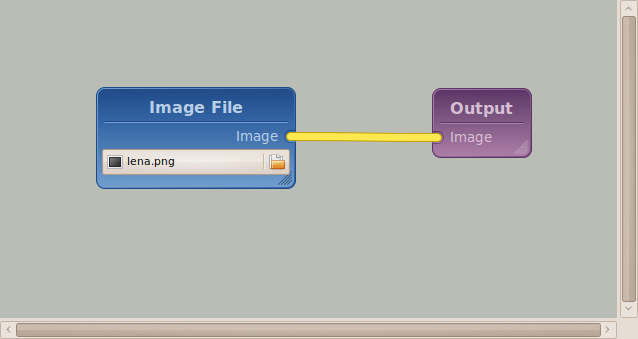
\includegraphics[width=\textwidth]{simple-pipeline}
\end{frame}

\begin{frame}
\lstinputlisting[language=Python,lastline=17]{examples/reduce/example1.py}
\end{frame}

\begin{frame}
\lstinputlisting[language=Python,firstline=19]{examples/reduce/example1.py}
\end{frame}

\begin{frame}
\begin{figure}\centering
\begin{tabular}{cc}
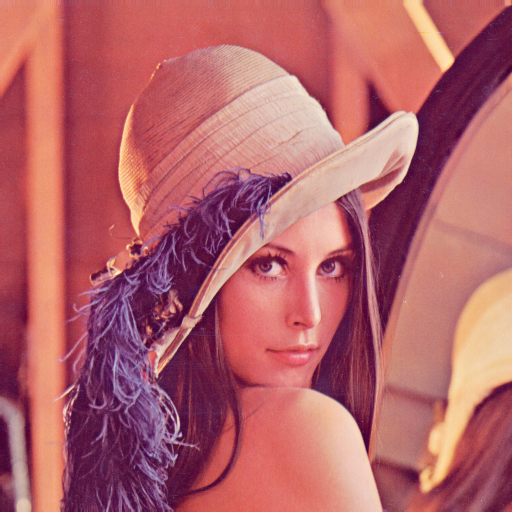
\includegraphics[width=0.4\textwidth]{examples/reduce/lena} &
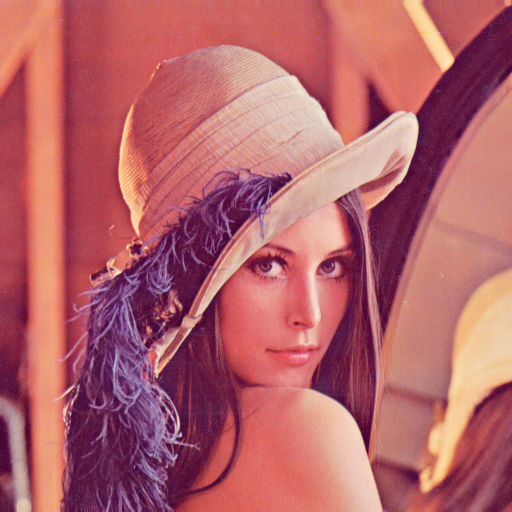
\includegraphics[width=0.4\textwidth]{examples/reduce/output_example1} \\
Input & Output
\end{tabular}
\end{figure}
\end{frame}

% }}}2

\section{Samplers} % {{{2

\begin{frame}{Samplers}
  \bi
    \item Know how to generate the red, green, blue and alpha components of
    an output pixel given its location
    \item Has an associated transform which maps from image-space co-ordinates
    to sampler-space co-ordinates
    \bi
      \item Allows transformation of images via a \emph{pass through} sampler
    \ei
    \item Black boxes but may depend on other samplers
    \item Supports three primitive operations
    \bi
      \item Prepare: Called once before the render
      \item Query: Called one or more times during the render
      \item Finish: Called once after the render
    \ei
  \ei
\end{frame}

% }}}2

\section{Sampler Types} % {{{2

\begin{frame}{Sampler Types}
  \bi
    \item A sampler is an abstract node
    \item Concrete implementations exist for various different images sources
    \item Buffer samplers sample from an in-memory image
    \bi
      \item Cairo surfaces, GdkPixbufs, images loaded by your own libraries
      (e.g.~The PIL), etc.
      \item Also a GStreamer plugin which uses a buffer sampler to provide
      video stream support
    \ei
    \item Kernel samplers use a small piece of code to generate the output
    pixel
    \bi
      \item The code may, itself, sample from other samplers
    \ei
    \item Advanced users can define their own samplers by implementing the
    three sampler primitives
  \ei
\end{frame}

% }}}2

\section{The Firtree Kernel Language} % {{{2

\begin{frame}{The Firtree Kernel Language}
  \bi
    \item The most interesting samplers are \emph{kernel samplers}
    \item A function which is called (conceptually) once per output pixel
    \item Returns the colour of a pixel given a \emph{destination co-ordinate}
    \item Language is based on a subset of C
    \item Extended with vectorised types
    \bi
      \item \texttt{a + b} $\rightarrow$ element-wise addition
      \item \texttt{a * b} $\rightarrow$ element-wise multiplication (not matrix
      multiplication)
    \ei
    \item Very similar to GLSL or CoreImage kernels
    \bi
      \item Inspired by CoreImage
      \item Originally implemented with the GLSL reference compiler
    \ei
  \ei
\end{frame}

% }}}2

\fancypart{Examples}

\section{Desaturate} % {{{2

\begin{frame}{Desaturate}
  \bi
    \item Convert an RGB image into the Y-component of a YUV image
    \item $Y = 0.299R + 0.587G + 0.114B$
    \item Use a simple kernel which uses the builtin \textbf{dot} function.
  \ei
\end{frame}

\begin{frame}
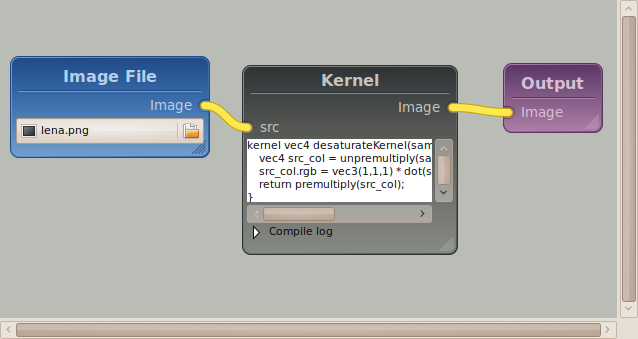
\includegraphics[width=\textwidth]{desat-pipeline}
\end{frame}

\begin{frame}
\lstinputlisting[language=Python,lastline=23]{examples/reduce/example2.py}
\end{frame}

\begin{frame}
\lstinputlisting[language=Python,firstline=25,lastline=47]{examples/reduce/example2.py}
\end{frame}

\begin{frame}
\lstinputlisting[language=Python,firstline=49]{examples/reduce/example2.py}
\end{frame}

\begin{frame}
\begin{figure}\centering
\begin{tabular}{cc}
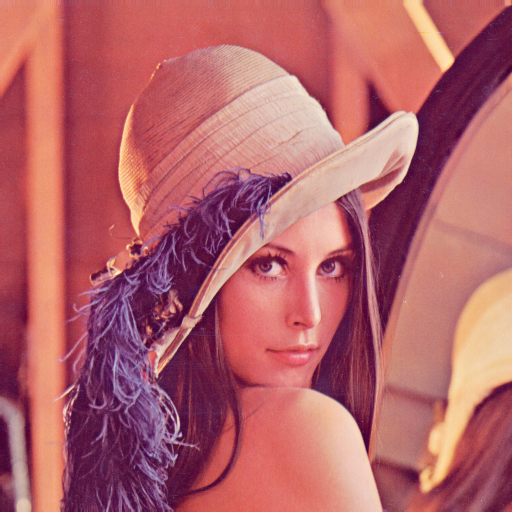
\includegraphics[width=0.4\textwidth]{examples/reduce/lena} &
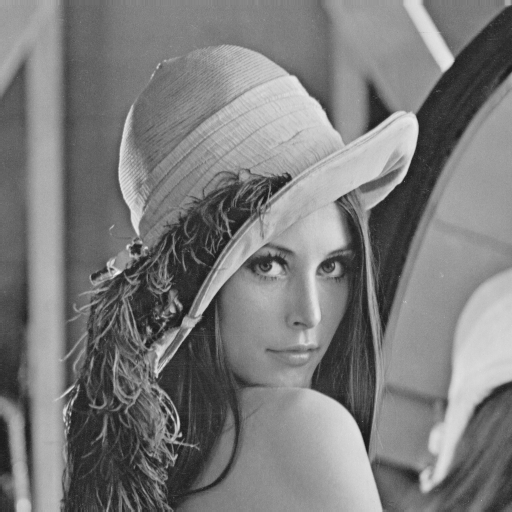
\includegraphics[width=0.4\textwidth]{examples/reduce/output_example2} \\
Input & Output
\end{tabular}
\end{figure}
\end{frame}

% }}}2

\section{Sobel Filter} % {{{2

\begin{frame}{Sobel Filter}
  \bi
    \item The Sobel Filter is a simple edge detector
    \item Convolves image with two kernels
    \[
    I_x = I * \left[
      \begin{array}{ccc}
      +1 & 0 & -1 \\
      +2 & 0 & -2 \\
      +1 & 0 & -1
      \end{array}
      \right] 
      \quad\mbox{and}\quad
      I_y = I * \left[
      \begin{array}{ccc}
      +1 & +2 & +1 \\
      0 & 0 & 0 \\
      -1 & -2 & -1
      \end{array}
      \right] 
    \]
    \item Computes edge response as $\sqrt{I_x^2 + I_y^2}$
    \item Need only append a kernel to the desaturate example above
  \ei
\end{frame}

\begin{frame}
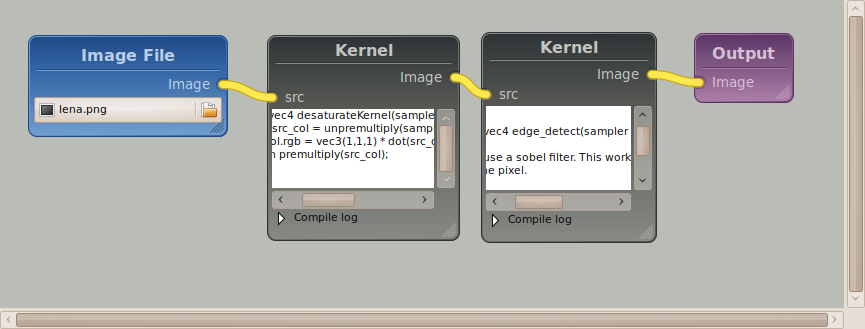
\includegraphics[width=\textwidth]{sobel-1-pipeline}
\end{frame}

\begin{frame}
\lstinputlisting[language=Python,firstline=47,lastline=50]{examples/reduce/example3.py}
\[ \cdots \]
\lstinputlisting[language=Python,firstline=87,lastline=87]{examples/reduce/example3.py}
\lstinputlisting[language=Python,firstline=89,lastline=89]{examples/reduce/example3.py}

\lstinputlisting[language=Python,firstline=100]{examples/reduce/example3.py}
\end{frame}

\begin{frame}
\lstinputlisting[language=Firtree,lastline=22]{examples/reduce/sobel.knl}
\end{frame}

\begin{frame}
\lstinputlisting[language=Firtree,firstline=24]{examples/reduce/sobel.knl}
\end{frame}

\begin{frame}
\begin{figure}\centering
\begin{tabular}{cc}
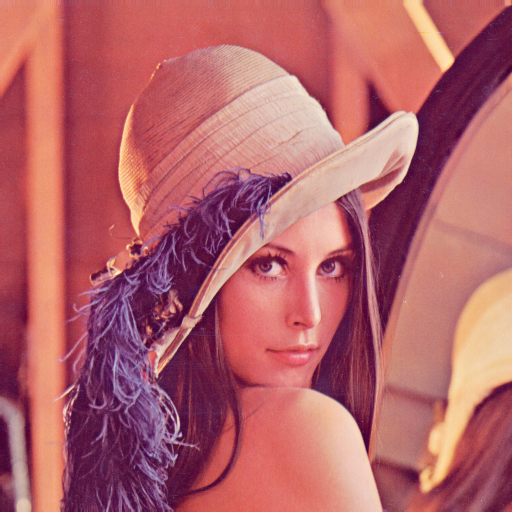
\includegraphics[width=0.4\textwidth]{examples/reduce/lena} &
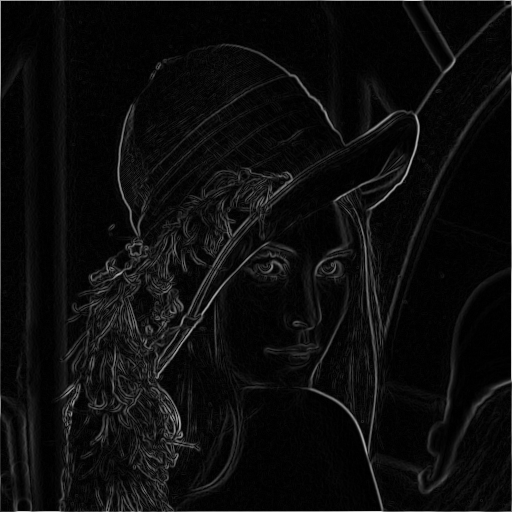
\includegraphics[width=0.4\textwidth]{examples/reduce/output_example3} \\
Input & Output
\end{tabular}
\end{figure}
\end{frame}

\begin{frame}{Extending Sobel Filter}
  \bi
    \item The Sobel kernel we defined earlier used 4-way vector arithmetic
    \item We can extend the program to give a colour output easily by simply
    'unplugging' the desaturate stage
    \item This requires precisely one line change:
    \lstinputlisting[language=Python,firstline=72,lastline=72]{examples/reduce/example4.py}
  \ei
\end{frame}

\begin{frame}
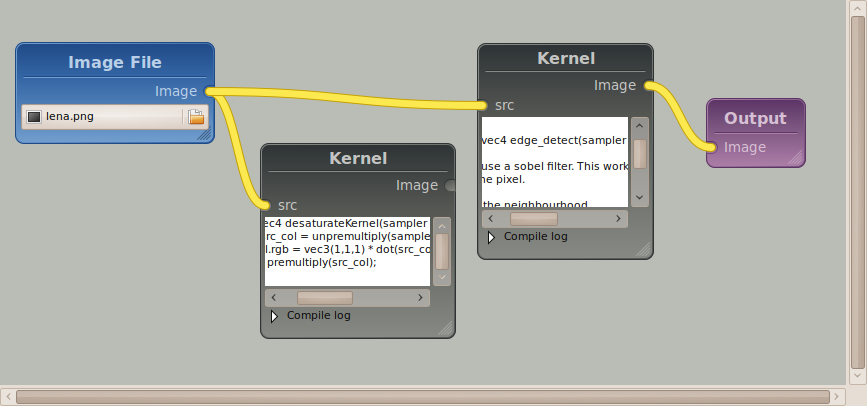
\includegraphics[width=\textwidth]{sobel-2-pipeline}
\end{frame}

\begin{frame}
\begin{figure}\centering
\begin{tabular}{cc}
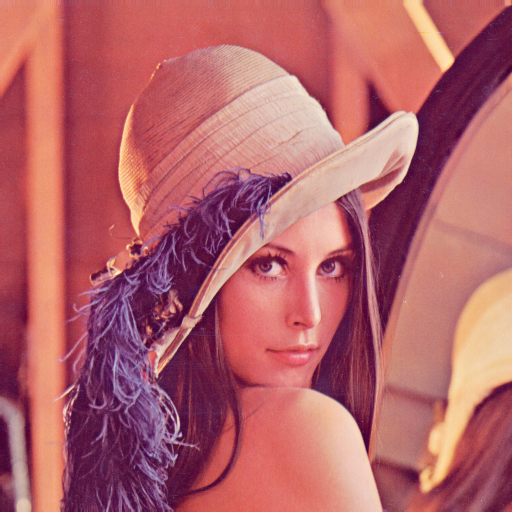
\includegraphics[width=0.4\textwidth]{examples/reduce/lena} &
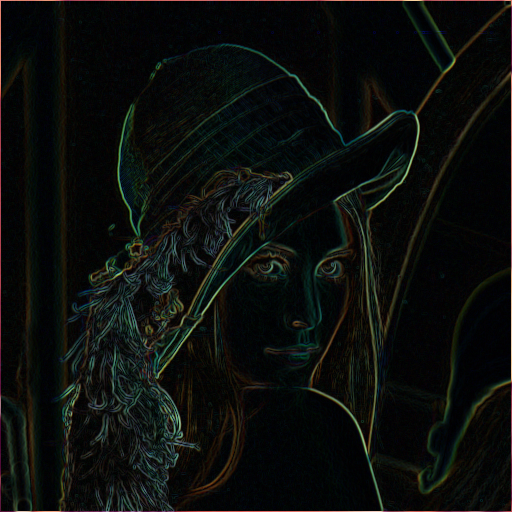
\includegraphics[width=0.4\textwidth]{examples/reduce/output_example4} \\
Input & Output
\end{tabular}
\end{figure}
\end{frame}

% }}}2

\section{Mandelbrot Set} % {{{2

\begin{frame}
\lstinputlisting[language=Python,firstline=25,lastline=26]{examples/mandelbrot.py}%
\lstinputlisting[language=Firtree,firstline=27,lastline=47]{examples/mandelbrot.py}%
\lstinputlisting[language=Python,firstline=48,lastline=48]{examples/mandelbrot.py}
\end{frame}

\begin{frame}
\lstinputlisting[language=Python,firstline=50]{examples/mandelbrot.py}
\end{frame}

\begin{frame}
\begin{figure}\centering
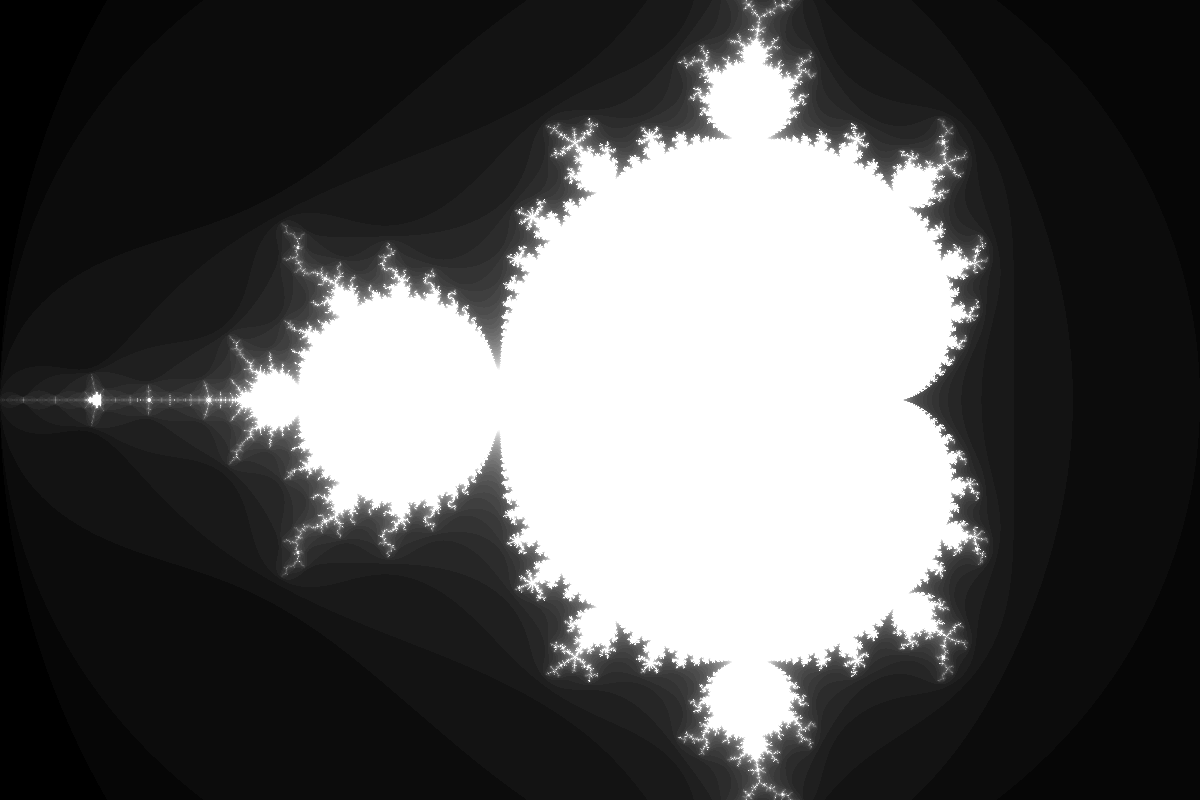
\includegraphics[width=\textwidth]{examples/mandelbrot} 
\caption{Output of \texttt{mandelbrot.py}}
\end{figure}
\end{frame}

% }}}2

\section{Reduce Kernels} % {{{2

\begin{frame}{Reduce Kernels}
  \bi
    \item Like normal image kernels except that they have no output
    \bi
      \item Kernel function returns \textbf{void}
      \item They cannot be associated with a sampler
    \ei
    \item Are conceptually called once per-pixel but in undefined order
    \item May make use of one extra builtin: \textbf{emit()}
    \bi
      \item Appends a \textbf{vec4} value to a global list
    \ei
    \item Somewhat misnamed; it is more of a selective filter + map
  \ei
\end{frame}

\begin{frame}
\lstinputlisting[language=Python,firstline=28,lastline=35]{examples/reduce/example6.py}
\end{frame}

\begin{frame}
\lstinputlisting[language=Python,firstline=86,lastline=103]{examples/reduce/example6.py}
\end{frame}

\begin{frame}
\lstinputlisting[language=Python,firstline=105]{examples/reduce/example6.py}
\end{frame}

\begin{frame}
\begin{figure}\centering
\begin{tabular}{cc}
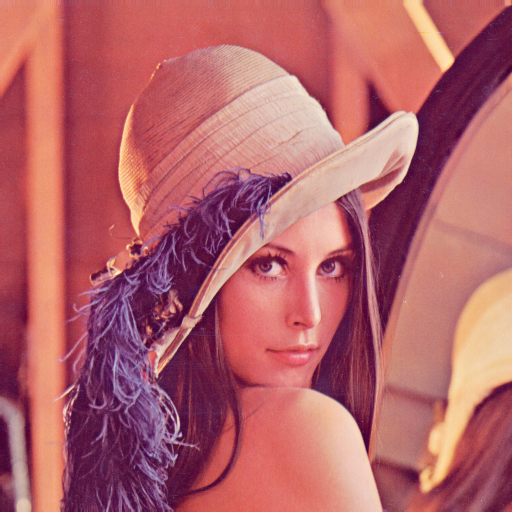
\includegraphics[width=0.4\textwidth]{examples/reduce/lena} &
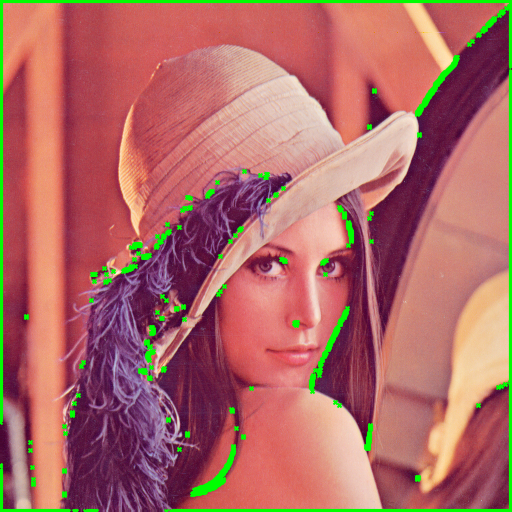
\includegraphics[width=0.4\textwidth]{examples/reduce/output_example6} \\
Input & Output
\end{tabular}
\end{figure}
\end{frame}

\begin{frame}
\lstinputlisting[language=Python,firstline=95]{examples/reduce/example7.py}
\end{frame}

\begin{frame}
\begin{figure}\centering
\begin{tabular}{cc}
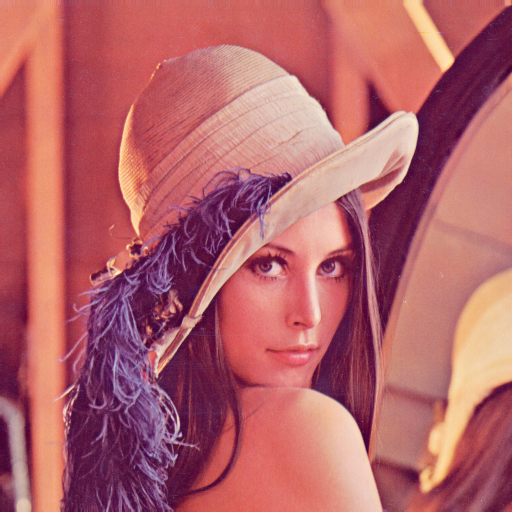
\includegraphics[width=0.4\textwidth]{examples/reduce/lena} &
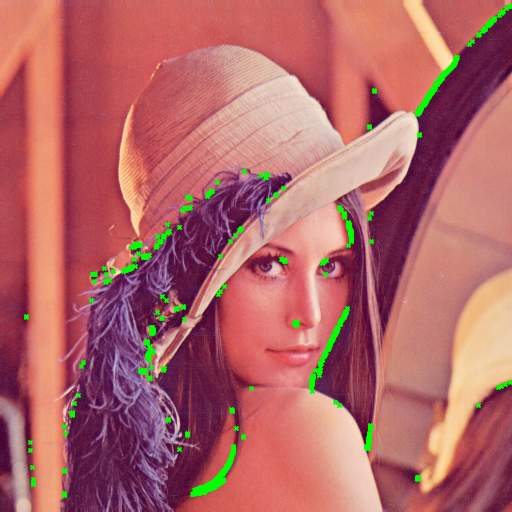
\includegraphics[width=0.4\textwidth]{examples/reduce/output_example7} \\
Input & Output
\end{tabular}
\end{figure}
\end{frame}

% }}}2

\section{Real-time Video Processing} % {{{2

\begin{frame}{Real-time Video Processing}
  \bi
    \item Sampler is sufficiently general that we can make a video source a
    sampler
    \item Have integrated Firtree with the GStreamer project
    \bi
      \item GStreamer allows one to create 'pluggable' modules that can decode
      video, camera streams, etc
    \ei
    \item Create a GStreamer \emph{sink} node which appears as a Firtree
    sampler
  \ei
\end{frame}

\begin{frame}
  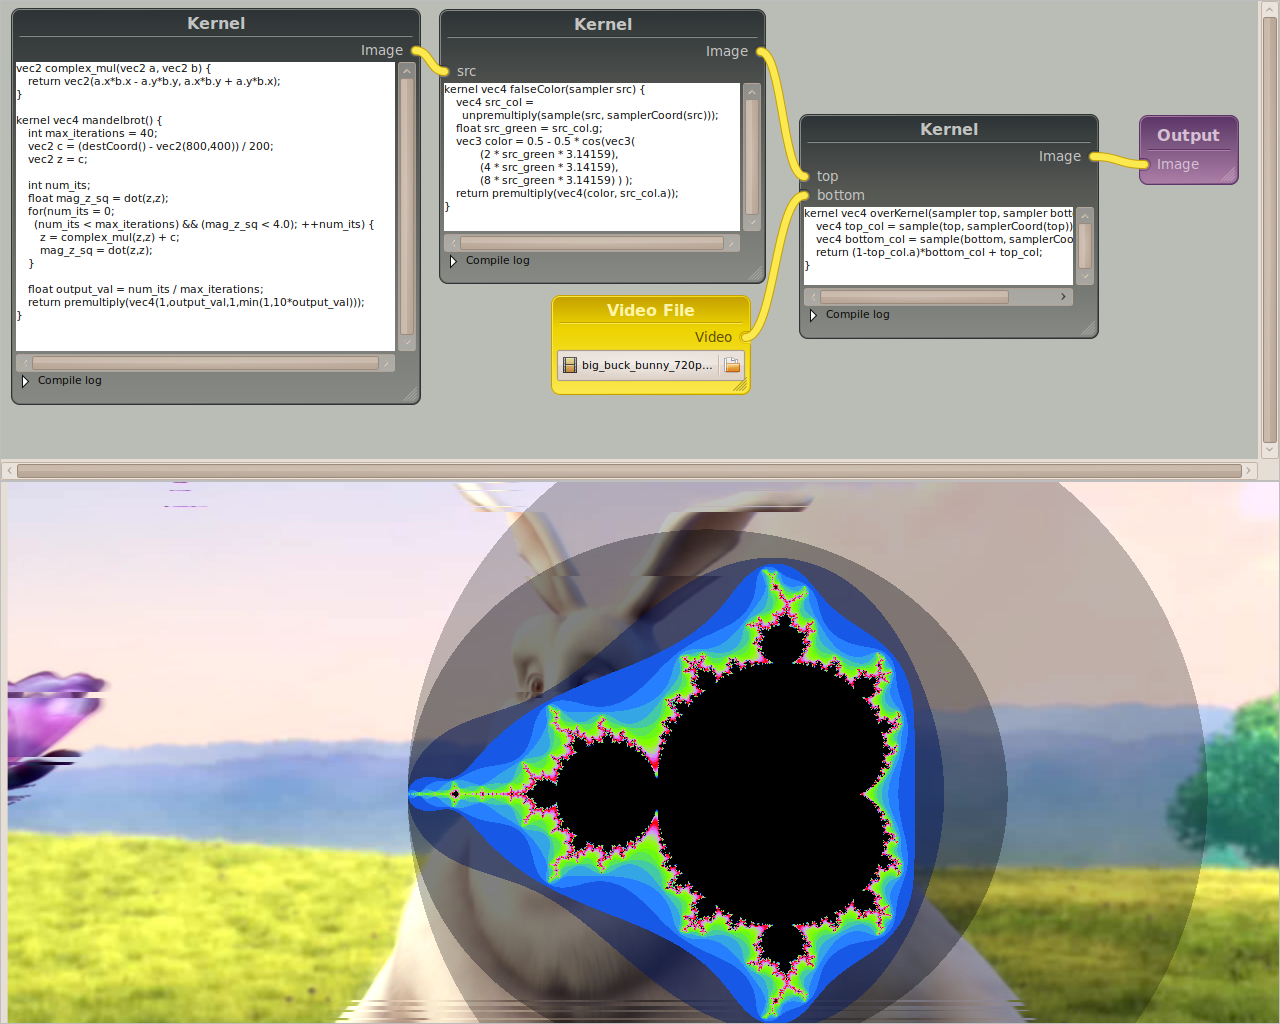
\includegraphics[width=\textwidth]{firtree-pipeline-image}
\end{frame}

% }}}2

\fancypart{Implementation}

\section{Compilation Process} % {{{2

\begin{frame}{Compilation Process}
  \bi
    \item Frontend compilation
    \bi
      \item Each sampler can represent its sampling action via a common
      Intermediate Representation (IR)
      \item IR has a number of low-level intrinsic functions
      \bi
        \item Sampling from image buffers, arithmetic operations,
        transcendental/trigonometric functions, etc.
      \ei
    \ei
    \item Backend execution
    \bi
      \item On first render, backend JIT compiles IR into native code
      \item Backend distributed work units to each compute unit
      \bi
        \item e.g.~CPU backend uses one thread per CPU which render blocks of
        output independently
      \ei
    \ei
  \ei
\end{frame}

\begin{frame}{Compilation Process (cont...)}
  \bi
    \item Each sampler generates IR for its action
    \item The IR linker automatically combines each sampler with the IR for
    its dependent samplers to produce a single block of IR
    \item The linking stage and those that precede it are backend independent
    \item The same IR may be passed to different backends if necessary
  \ei
\end{frame}

% }}}2

\section{LLVM} % {{{2

\begin{frame}{LLVM}
  \bi
    \item Make use of the IR from the LLVM project\footnote{http://llvm.org/}
    \item Provides an in-memory and human-readable variant
    \item Includes a suite of modern optimisation stages
    \item Includes native vector-aware backends for most modern CPUs
    \item nVidia have a backend which targets their compute-capable graphics
    cards
  \ei
\end{frame}

\begin{frame}{LLVM Example}
  \bi
    \item Use the simple identity pipeline example
    \lstinputlisting[language=Python,firstline=10,lastline=11]{examples/reduce/example1.py}
    \item Sampler generates following IR
    \scalebox{0.75}{\lstinputlisting[language=llvm]{examples/reduce/example1_asm.txt}}
  \ei
\end{frame}

\begin{frame}
    \lstinputlisting[language=Firtree]{examples/sin-kernel.knl}
    \lstinputlisting[language=llvm]{examples/sin-asm.txt}
\end{frame}

\begin{frame}
  \begin{figure}\centering
  
\includegraphics[height=\textheight]{examples/sin-example}
  \end{figure}
\end{frame}

% }}}2

\section{Sampler Linking} % {{{2

\begin{frame}{Sampler Linking}
  \bi
    \item Samplers may call other samplers
    \lstinputlisting[language=Firtree]{examples/sin-example-2.knl}
    \item Kernel is compiled into IR which makes use of sampler functions
  \ei
\end{frame}

\begin{frame}
    \lstinputlisting[language=Firtree]{examples/sin-kernel.knl}
    \scalebox{0.8}{\lstinputlisting[language=llvm]{examples/sin-image-kernel-asm.txt}}
\end{frame}

\begin{frame}{Linker Output}
  Setting lena as \texttt{src} causes the linker to inline calls to
  the sampler:
  \scalebox{0.75}{\lstinputlisting[language=llvm]{examples/sin-asm-2.txt}}
\end{frame}

\begin{frame}
  \begin{figure}\centering
  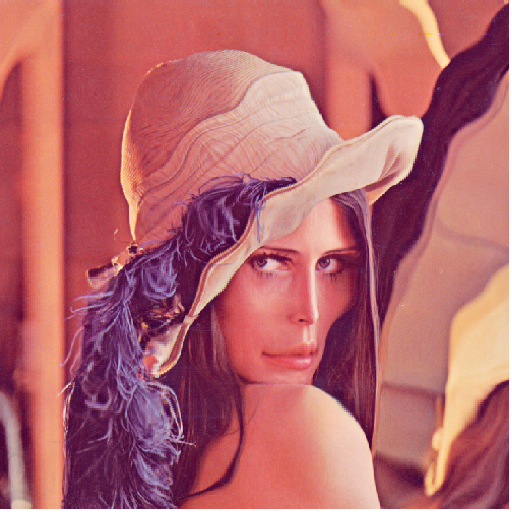
\includegraphics[height=\textheight]{examples/sin-example-2}
  \end{figure}
\end{frame}
% }}}2

\section{Backends} % {{{2

\begin{frame}{Backends}
  Backends are responsible for platform specific tasks:
  \bi
    \item Compiling LLVM IR to native code
    \item Implementing the intrinsics
    \item Distributing rendering onto multiple cores
  \ei
\end{frame}

% }}}2

\subsection{Multi-core CPU} % {{{2

\begin{frame}{The CPU backend}  
  \bi
    \item Wraps the sampler IR in LLVM IR which implements an inner rendering
    loop
    \bi
      \item Similar to the plain C example at the start of the talk
    \ei
    \item Maintains one worker thread per-CPU
    \item Divides rendering task into small chunks
    \item Each worker thread gets a new chunk from a global queue
    \item Easier parts of the image do not cause threads to become idle
  \ei
\end{frame}

\begin{frame}
  The generated CPU assembly (x86 in this case) can be quite daunting
  \vfill
  \begin{columns}
    \column{0.33\textwidth}
    \scalebox{0.3}{\lstinputlisting[basicstyle=\tiny\ttfamily,lastline=74]{examples/simple-x86.txt}}
    \column{0.33\textwidth}
    \scalebox{0.3}{\lstinputlisting[basicstyle=\tiny\ttfamily,firstline=75,lastline=148]{examples/simple-x86.txt}}
    \column{0.33\textwidth}
    \scalebox{0.3}{\lstinputlisting[basicstyle=\tiny\ttfamily,firstline=149]{examples/simple-x86.txt}}
  \end{columns}
\end{frame}

% }}}2

\subsection{The future: GPU} % {{{2

\begin{frame}{The future: GPU}
  \bi
    \item Post Firtree re-write GPU renderer has not been re-implemented
    \item A proof-of-concept LLVM IR to OpenCL/CUDA converter exists
    \item Not yet fully implemented
    \bi
      \item Very small number of intrinsics
      \item Does not execute the code it compiles
    \ei
    \item Waiting for an excuse to implement it
    \item Some interesting issues arise
    \bi
      \item Backend will also have to maintain buffer cache on compute card
      \item Want to create some render \emph{queue} so that entire rendering
      pipeline becomes asynchronous
    \ei
  \ei
\end{frame}

\begin{frame}{The past: GPU}
  \bi
    \item An earlier version of Firtree had a GPU backend
    \item Was based on OpenGL + GLSL
    \item The 'unique' way OpenGL contexts are managed caused it to be brittle
    \item Was very fast indeed
    \item Even compute-intensive kernels required negligible CPU
    \item Some pretty videos were generated
  \ei
\end{frame}

% }}}2

\begin{frame}
  \begin{figure}\begin{centering} 
    \Huge Questions?
  \end{centering}\end{figure}
\end{frame}

\end{document}

% vim:spell:spelllang=en_gb:ts=2:sw=2:et:autoindent:foldmethod=marker:foldlevel=1:tw=78
